\documentclass{article}

\usepackage{amsmath}
\usepackage{tabularx}
\usepackage[table]{xcolor}
\usepackage{hyperref}
\usepackage{cleveref}
\usepackage{tikz}
\usetikzlibrary{positioning, calc, shapes, arrows, fit}
\usepackage{circuitikz}
\usepackage{subcaption}
\usepackage[colorinlistoftodos]{todonotes}
\linespread{0.9}
\hypersetup{
    colorlinks = true,
    citecolor = black,
    linkcolor = black,
}

\begin{document}
\title{Lab 3 -- Exploring the diode-ring mixer}
\author{
    Yifan Zhu\\
    Lab Partner: John Kustin
}
\maketitle

\begin{abstract}
\end{abstract}

\section{Introduction}
Mixers are three-port devices (\Cref{fig:mixer}) that produce sum and difference frequencies of the two supplied input frequencies.
They have wide applications including use as modulators, phase detectors, and product detectors.

\begin{figure}[h]
    \centering
    \begin{circuitikz}
        \draw node[mixer] (mix) {};
        \draw[<-] (mix) -- ++(2, 0) node[midway, label=RF] {};
        \draw[<-] (mix) -- ++(-2, 0) node[midway, label=LO] {};
        \draw[->] (mix) -- ++(0, 2) node[midway, label=right:IF] {};
    \end{circuitikz}
    \caption{Mixer}
    \label{fig:mixer}
\end{figure}

Typically, one of the inputs to the mixer is a local oscillator (LO), and for down conversion, the other input signal is called RF, and the output is called IF (intermediate frequency).

In this lab we build a diode-ring mixer, and test its various characteristics.
The diode-ring mixer is a passive, double balanced mixer.
The passive design allows for greater bandwidth, at the cost of greater conversion loss;
and the double balanced design provides great RF and LO supression.

\section{Experimental Setup}
\tikzset{circ_e/.style={
            circ,
            draw,
            inner sep=1pt,
            shape=circle
        }}
\tikzset{full diode/.append style={
            /tikz/every node/.append style={/tikz/scale=0.5}
        }
}

\begin{figure}[h]
    \centering
    \begin{circuitikz}[transform shape]
        \draw[short] (0,0) to ++(8, 0);
        \draw (1, 0) to[short, *-] ++(0, 1.5)
        to[inductor] ++(0, 1)
        to[short] ++(0, 1)
        to[short] ++(-1, 0) node[circ_e, label=LO] {};
        \draw (2, 0.5) to[inductor] ++(0, 1.5)
        to[inductor] ++(0, 1.5);
        \draw (2, 2) to[short, *-] ++(0.5, 0)
        to[short, -*] (2.5, 0);

        \draw (3, 2) to[full diode, -*] ++(1, 1)
        to[full diode, -*] ++(1, -1)
        to[full diode, -*] ++(-1, -1)
        to[full diode, -*] ++(-1, 1)
        ;
        \draw[short] (2, 3.5) -| (4, 3);
        \draw[short] (2, 0.5) -| (4, 1);

        \draw (6, 1) to[inductor] ++(0, 1.5)
        to[inductor] ++(0, 1.5);
        \draw (6, 2.5) to[short, *-] ++(-0.5, 0)
        to[short] (5.5, 0.5) node[circ_e, label=right:IF] {};
        \draw (5.5, 0) to[short] ++(0, 0.1) node[circ_e, label] {};

        \draw[short] (6, 4) -| (3, 2);
        \draw[short] (6, 1) -| (5, 2);

        \draw (7, 0) to[short, *-] ++(0, 2)
        to[inductor] ++(0, 1)
        to[short] ++(0, 1)
        to[short] ++(1, 0) node[circ_e, label=RF] {};
    \end{circuitikz}
    \caption{Circuit of Double Balanced Diode Ring Mixer}
    \label{fig:mixer_circuit}
\end{figure}

We build the double balanced diode ring mixer according to \Cref{fig:mixer_circuit}.
It consists of two transformers and a diode ring.
The ring diode used is \href{https://www.infineon.com/dgdl/Infineon-BAT15-099R-DS-v01_00-EN.pdf?fileId=5546d46265f064ff0166389632964e8c}{BAT15-099R}, which can be used in these mixers for up to 12GHz in frequency.
The RF transformers are \href{https://www.minicircuits.com/pdfs/ADT4-1WT+.pdf}{ADT4-1WT+}, which work from 2 to 775 MHz.
Here, the transformers are used as baluns, which convert between balanced and unbalanced signals.

\section{Results and Discussion}
\subsection{Overall Performance}
To test our mixer, we drove both the LO and RF inputs at 0dBm, and set RF frequency to 10MHz, and LO frequency to 7.1MHz.
The output spectrum from 0Hz to 40MHz is shown in \Cref{fig:mixer_out}, where the sum and difference frequencies, as well as the most prominent intermodulation distortions are marked by texts.

\tikzset{annotation/.style={color=yellow, scale=.5, align=center}}
\begin{figure}[h]
    \centering
    \begin{tikzpicture}[scale=0.9, transform shape]
        \node[anchor=south west, inner sep=0] (X) at (0,0){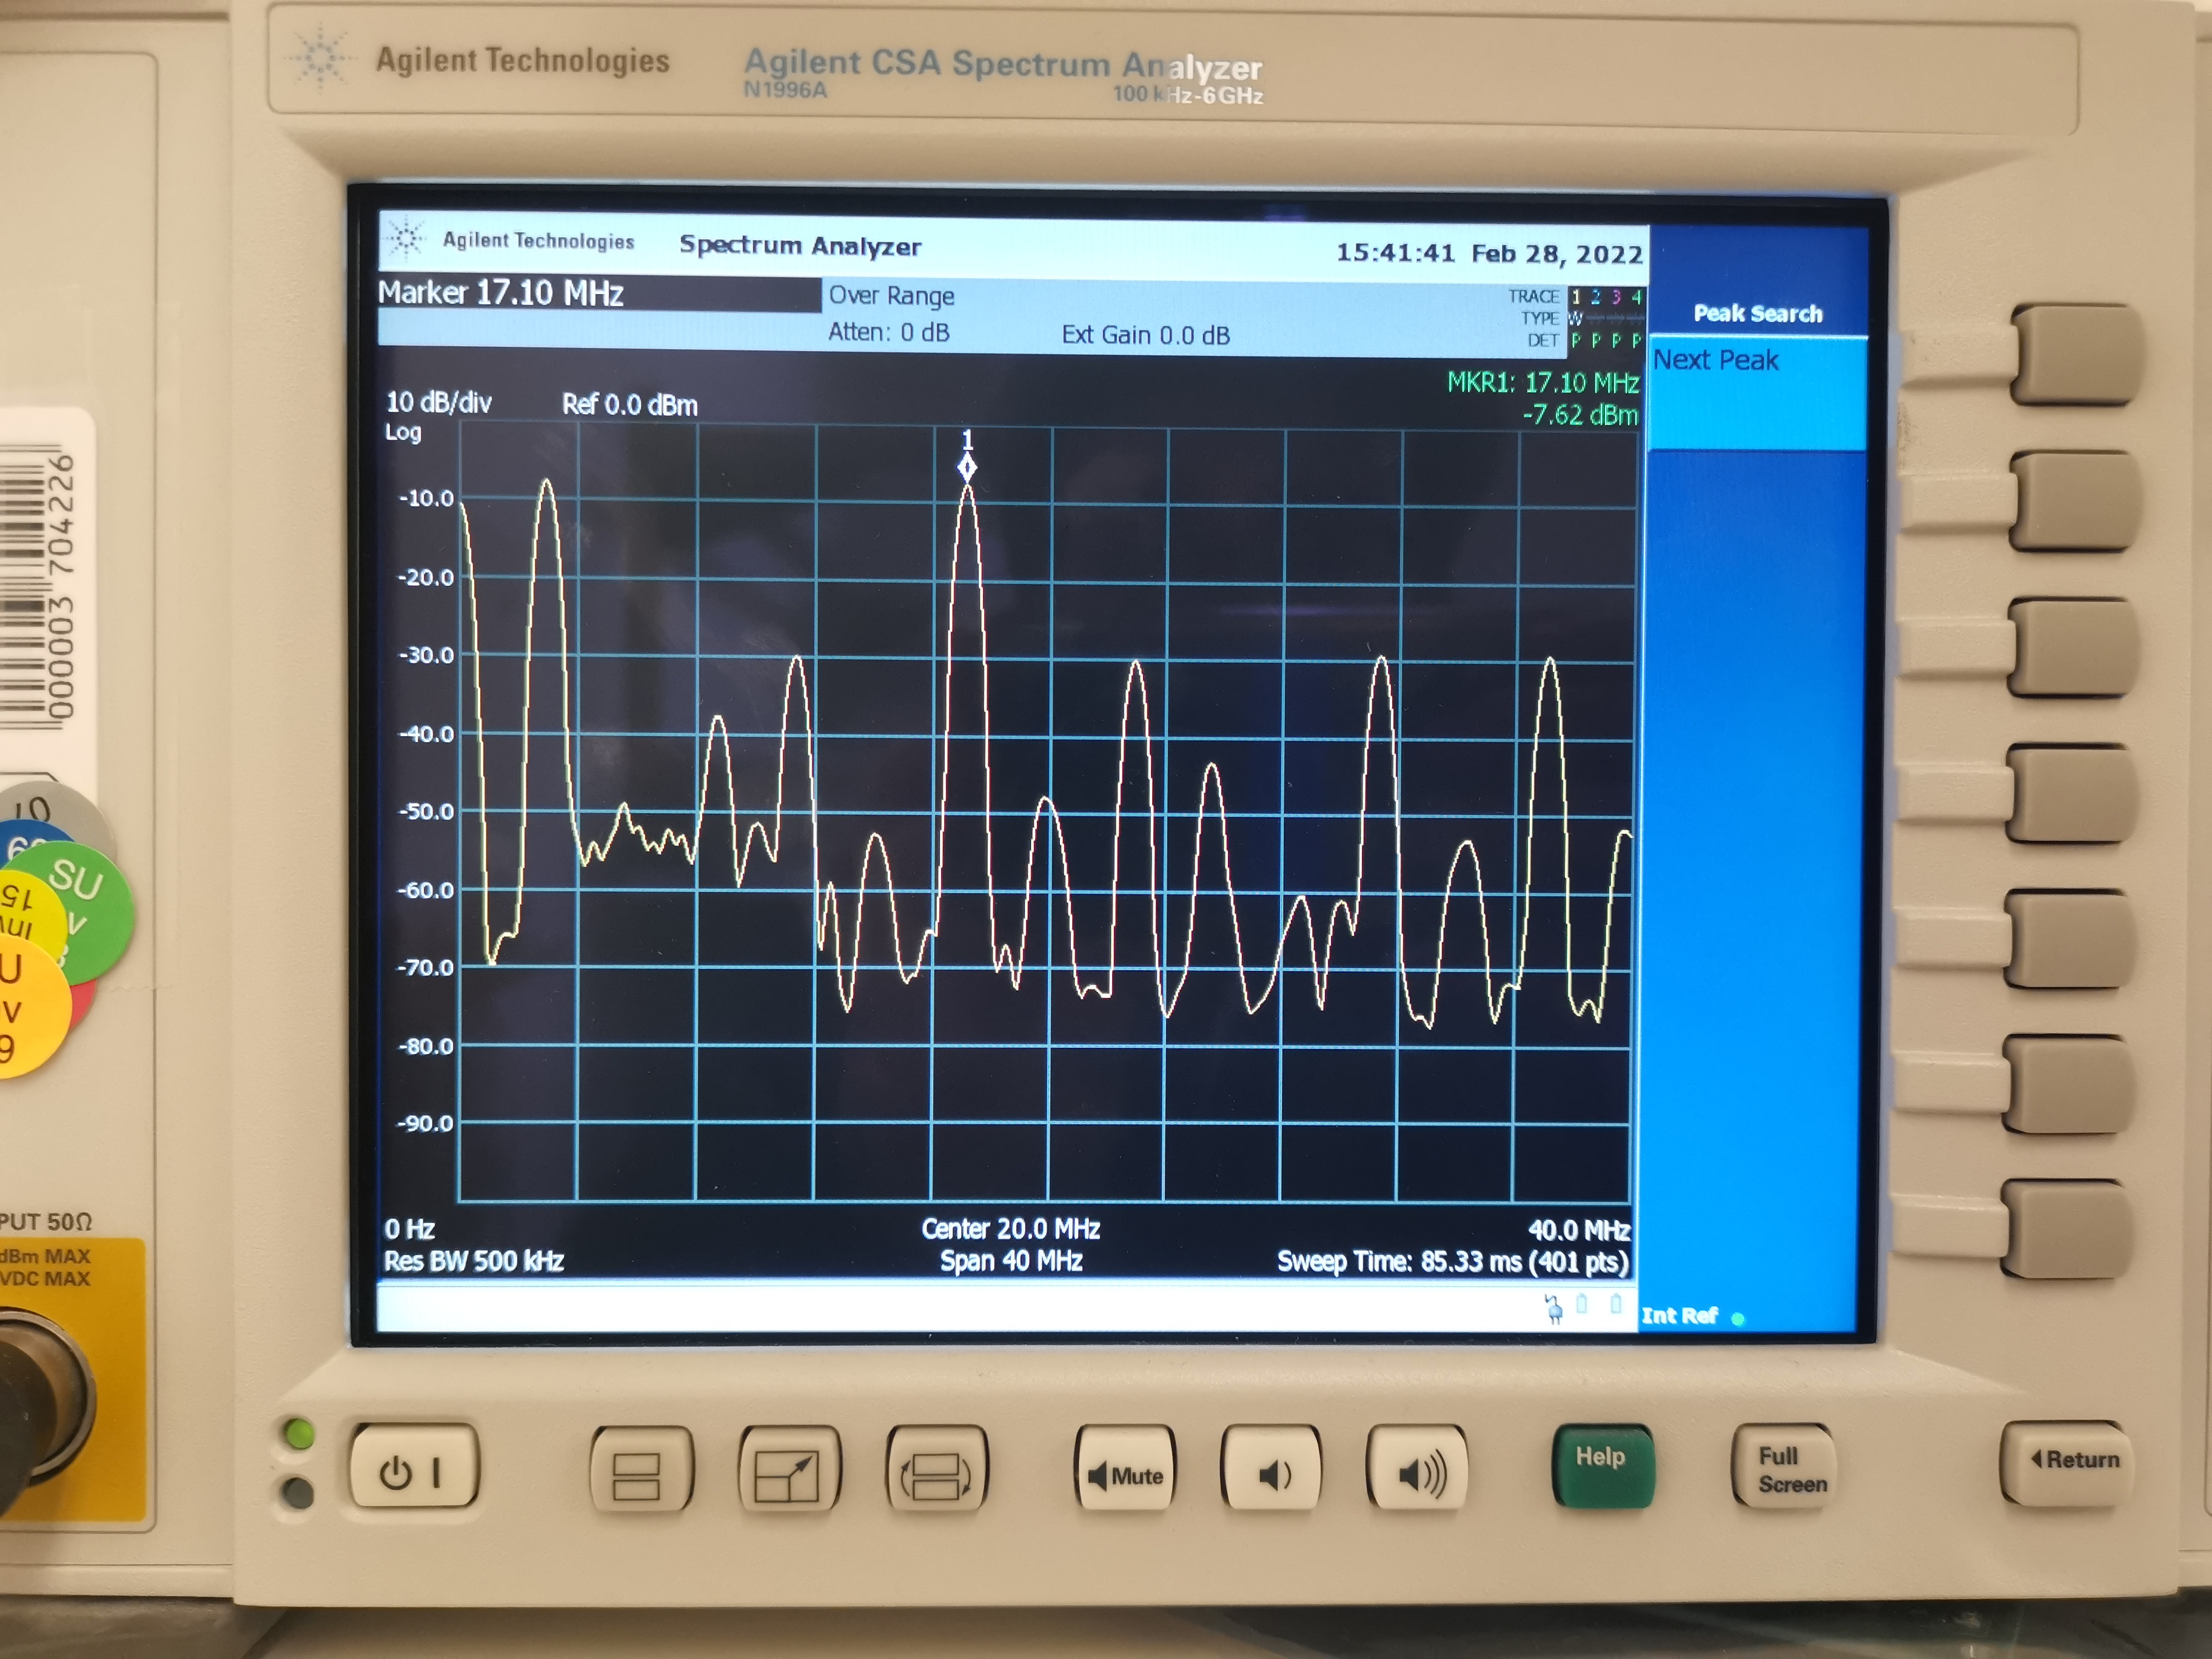
\includegraphics[width=\textwidth]{./pics/mixer_out_RF10_LO7_1.jpg}};% 
        \node[annotation] at (3, 6) {RF-LO\\2.9MHz};
        \node[annotation] at (5.3, 6) {RF+LO\\17.1MHz};
        \node[annotation] at (7.65, 5.7) {RF+3LO\\31.3MHz};
        \node[annotation] at (4.36, 5.7) {-RF+3LO\\11.3MHz};
        \node[annotation] at (8.60, 5.7) {3RF+LO\\37.1MHz};
        \node[annotation] at (6.27, 5.7) {3RF-LO\\22.9MHz};
    \end{tikzpicture}
    \caption{Spectrum of Mixer Output. LO=RF=0dBm.}
    \label{fig:mixer_out}
\end{figure}

From the figure, we can see that both the sum (17.1MHz) and different (2.9MHz) frequencies are at least 20dB above the intermodulation distortions, which means our mixer mixes the two inputs pretty well.
In addition, the LO leakage is virtually non-existant -- well below -50dB at 7.1MHz.

Interestingly, at this level of input, the highest spurs occur at $3RF\pm LO$ and $3LO \pm RF$.
These are all fourth-order intermodulations, with odd orders for both the RF and the LO componenets.
We hypothesize that this particular diode-ring mixer network suppresses intermodulations when either the RF or the LO has even orders.
To validate this hypothesis, we lowered RF to -10dBm, while keeping LO at 0dBm.
The results are shown in \Cref{fig:mixer_out_2}.

\begin{figure}[h]
    \centering
    \begin{tikzpicture}[scale=0.9, transform shape]
        \node[anchor=south west, inner sep=0] (X) at (0,0){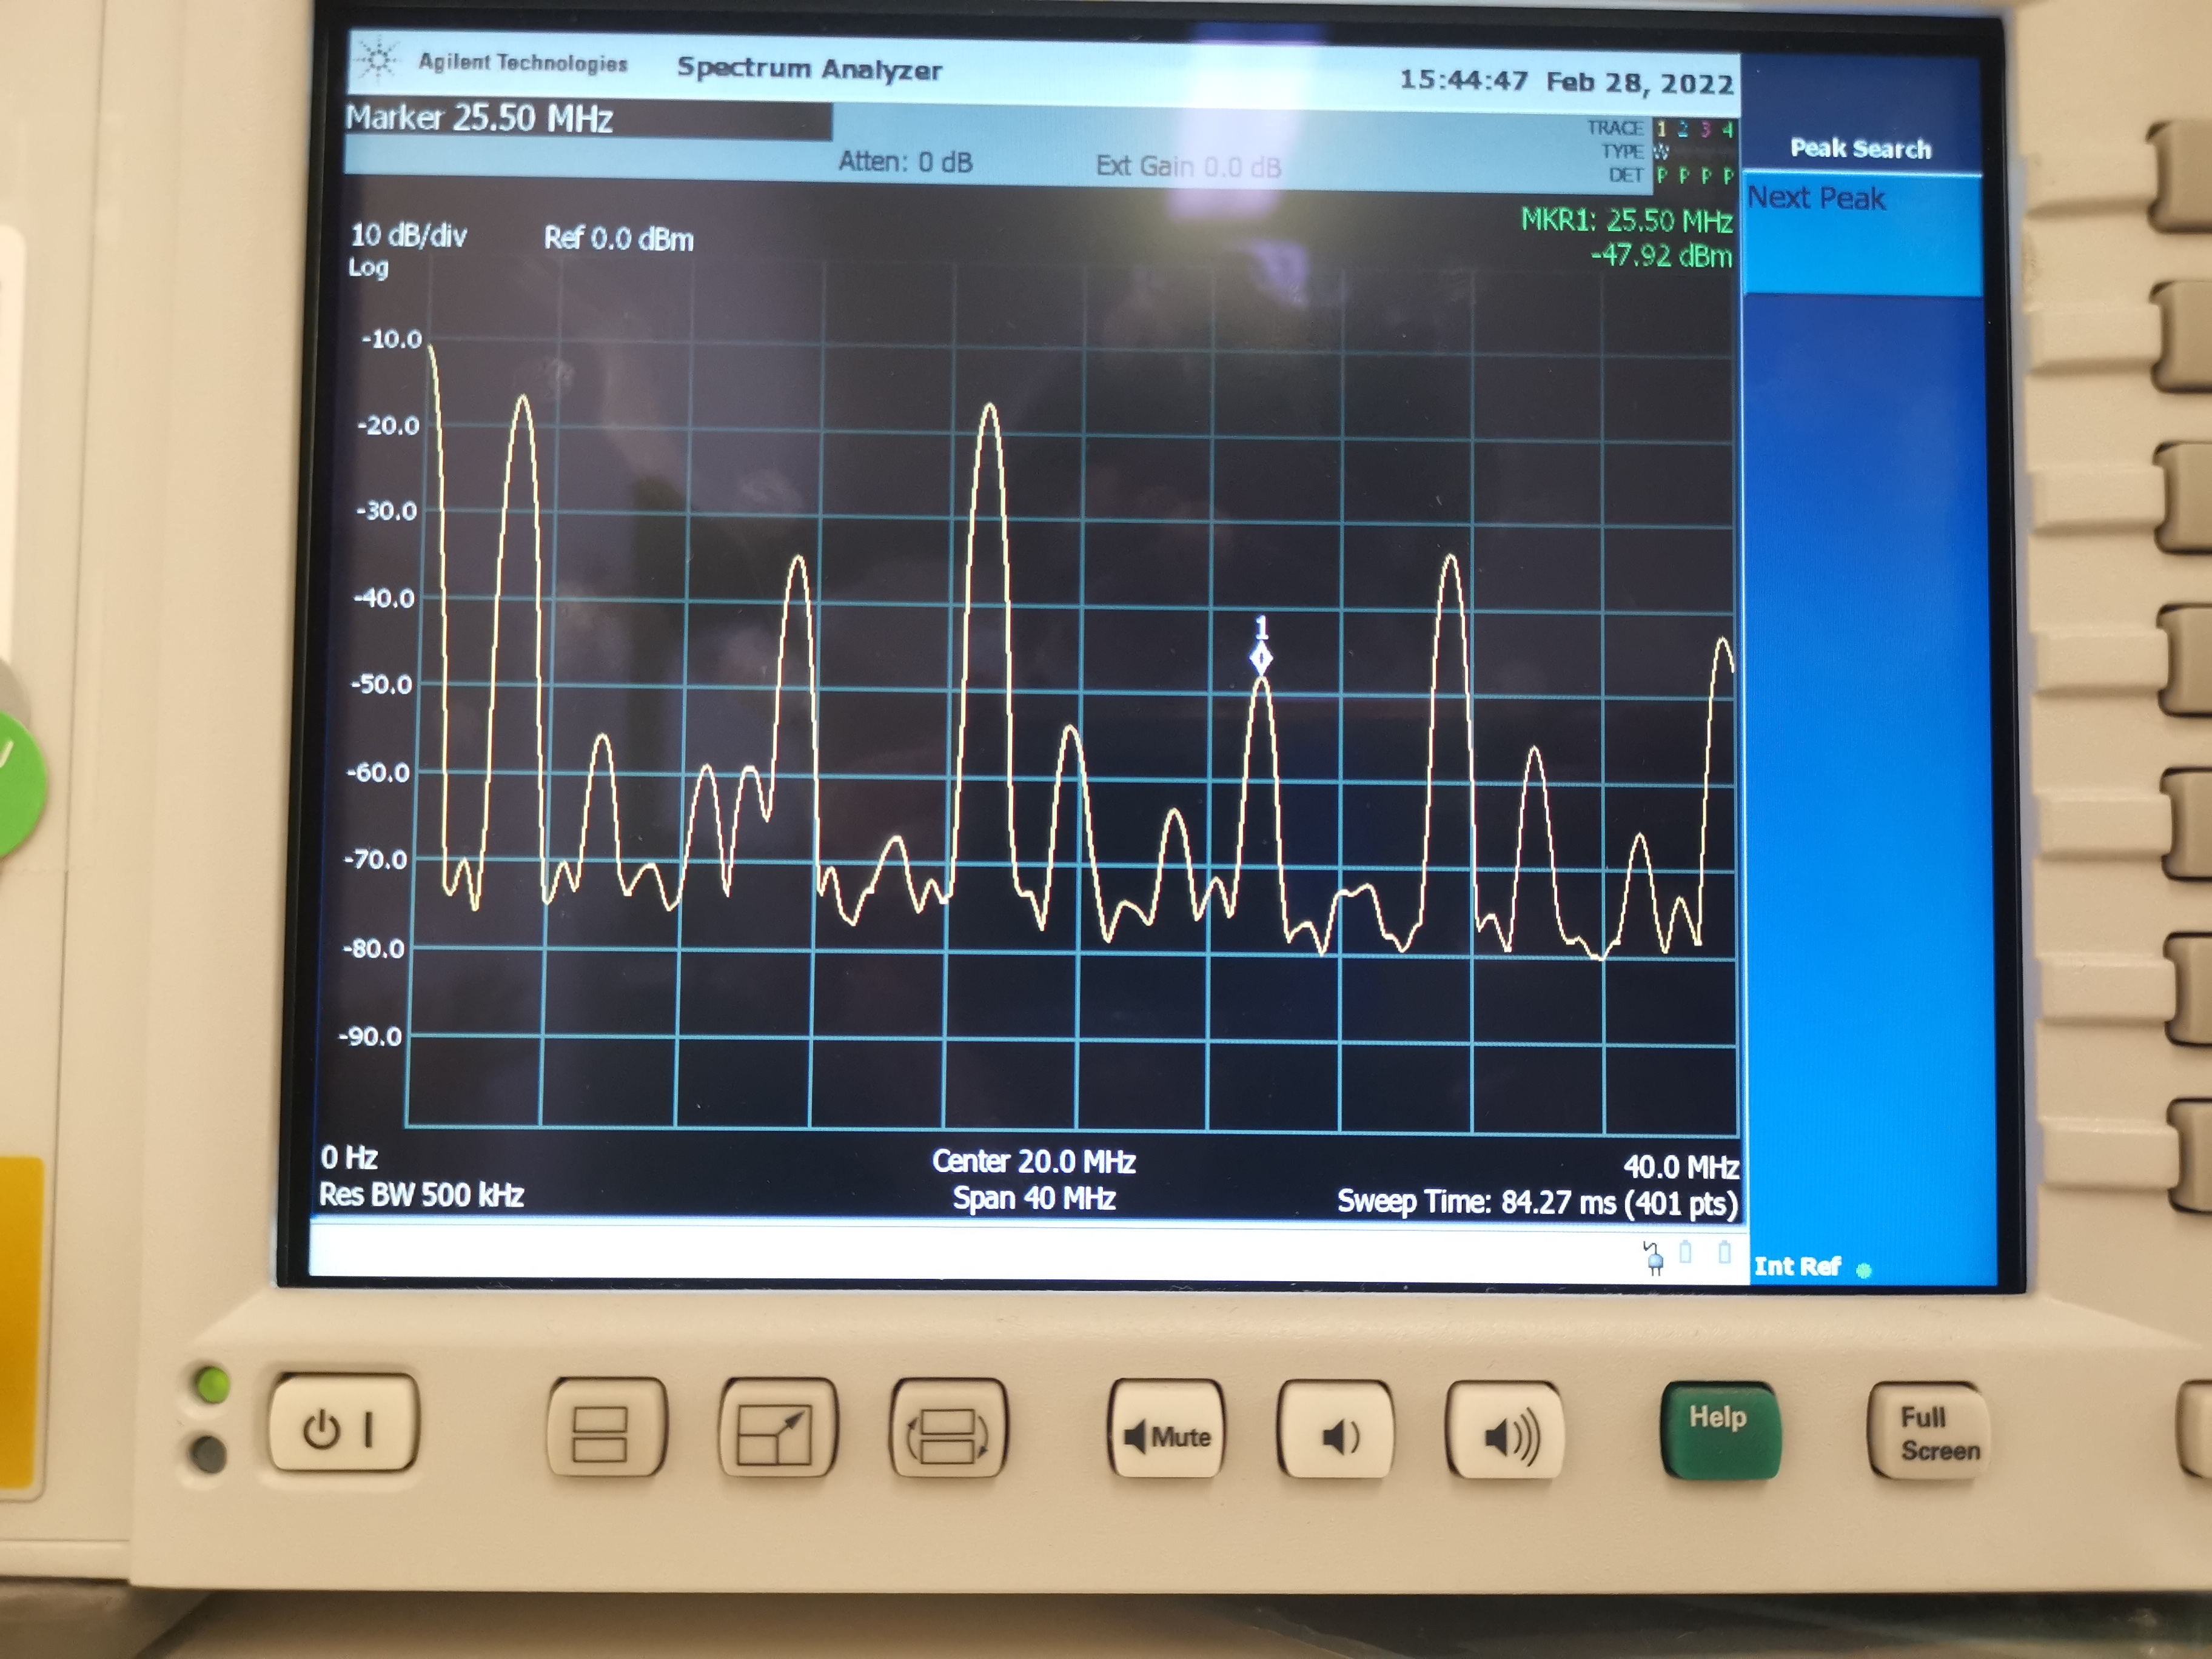
\includegraphics[width=\textwidth]{./pics/mixer_out_RF10_LO7_1_2.jpg}};% 
        \node[annotation] at (2.85, 6.2) {RF-LO\\2.9MHz};
        \node[annotation] at (5.43, 6.2) {RF+LO\\17.1MHz};
        \node[annotation] at (8.09, 6.2) {RF+3LO\\31.3MHz};
        \node[annotation] at (4.41, 6.2) {-RF+3LO\\11.3MHz};
        \node[annotation] at (7.00, 6) {-RF+5LO\\25.5MHz};
        \node[annotation] at (9.44, 6) {8RF-13LO\\39.7MHz};
    \end{tikzpicture}
    \caption{Spectrum of Mixer Output. LO=0dBm, RF=-10dBm.}
    \label{fig:mixer_out_2}
\end{figure}

In this case, the biggest intermodulations are at $3LO\pm RF$, $5LO-RF$, and something at 39.7MHz, which seems to be $8RF-13LO$.
The $5LO-RF$ still confirms our hypothesis of the mixer suppressing even orders of LO and RF.
The component at 39.7MHz is quite weird, and we have no idea why this intermodulation would be so big.

\subsection{Conversion Gain and 1dB Compression Point}
An important performance metric of mixers is the conversion gain, defined as the power level of the IF output minus the power level of the RF input in dBs.
Ideally, the conversion gain would be constant at all RF input levels.
However, for real mixers, as the RF input power increases, the IF output power cannot keep up with the increase in input.
The point where the ideal output power is 1dB lower than the actual output power is called the 1dB compression point.

We measured the 1dB compression point and gain when LO=0dBm by stepping the RF input power from -10dBm to 0dBm.
The results are plotted in \Cref{fig:rf_if}.

\begin{figure}
    \centering
    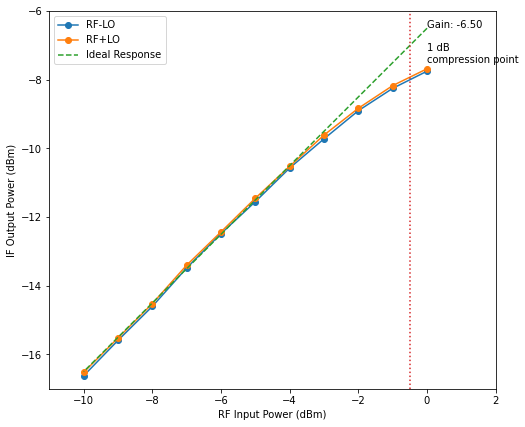
\includegraphics[width=0.5\linewidth]{./pics/1db_compression.png}
    \caption{RF Input Power vs IF Output Power (LO=0dBm)}
    \label{fig:rf_if}
\end{figure}

From the figure, we can see that under -4dBm, the relationship between input power and output power (in dBs) is very linear, with gain around $-6.5dB$.
Ideally, the diode ring passive mixer would equally divide all the input power between the sum and the difference frequencies in the output.
So we would expect to see a gain of $-6dB$ for both.
The $0.5dB$ discrepancy between the measured $-6.5dB$ and the theoretical $0.5dB$ is probably due to non-ideal componenents.

However, above $-4dBm$, the ideal response and actual response start to differ, and we reach the 1dB compression point around $-0.5dBm$.

\subsection{Conversion Gain vs LO Drive Level}

\subsection{Third-Order Intercept}

\subsection{Port Isolations}

\section{Conclusions}
Learn more about why some harmonics are more prominant
\end{document}